\section{Naive Bayes classifier}

% ----- Q.1 ----- %
\subsection{The Naive Bayes classifier prediction}
Let $y$ be the class variables and $\bm{x} = (x_1, x_2, ...)$ the dependent input variables.\par
Bayes' theorem states that
\begin{equation*}
    P\left(y | x_{1}, \ldots, x_{n}\right) = \frac{P(y) P\left(x_{1}, \ldots x_{n} | y\right)}{P\left(x_{1}, \ldots, x_{n}\right)}
\end{equation*}
Knowing that
\begin{equation*}
    P\left(x_{1}, \ldots, x_{n}\right | y) = \prod_{i=1}^{n} P\left(x_{i} | y, x_{1}, \ldots, x_{i-1}\right)
\end{equation*}
and that the $x_i$ are conditionally independent given the output (the {\it naive Bayes independance assumption}), {\it i.e.}
\begin{equation*}
    P\left(x_{i} | y, x_{1}, \ldots, x_{i-1}, x_{i+1}, \ldots, x_{n}\right) = P\left(x_{i} | y\right)
\end{equation*}
we can write
\begin{equation*}
    P\left(y | x_{1}, \ldots, x_{n}\right) = \frac{P(y) \prod_{i=1}^{n} P\left(x_{i} | y\right)}{P\left(x_{1}, \ldots, x_{n}\right)}
\end{equation*}
The denominator being constant given $y$, we can finally write
\begin{align*}
    \hat{f}(\mathbf{x}) &= \operatorname{argmax}_{y} \operatorname{P}\left(y | x_{1}, \ldots, x_{n}\right)\\
    &= \operatorname{argmax}_{y} \operatorname{P}(y) \prod_{i=1}^{n} \operatorname{P}\left(x_{i} | y\right)
\end{align*}

% ----- Q.3 ----- %
\setcounter{subsection}{2}
\subsection{Testing set accuracy}
We used our own naive Bayes estimator on both datasets. To illustrate our results, we present the decision boundary of each dataset at figure \ref{fig:gnb}.\par
In order to make the visualization clearer, we only displayed \num{25}\% of the points of each testing set.
\begin{figure}[H]
    \centering
    \begin{subfigure}{0.495\textwidth}
        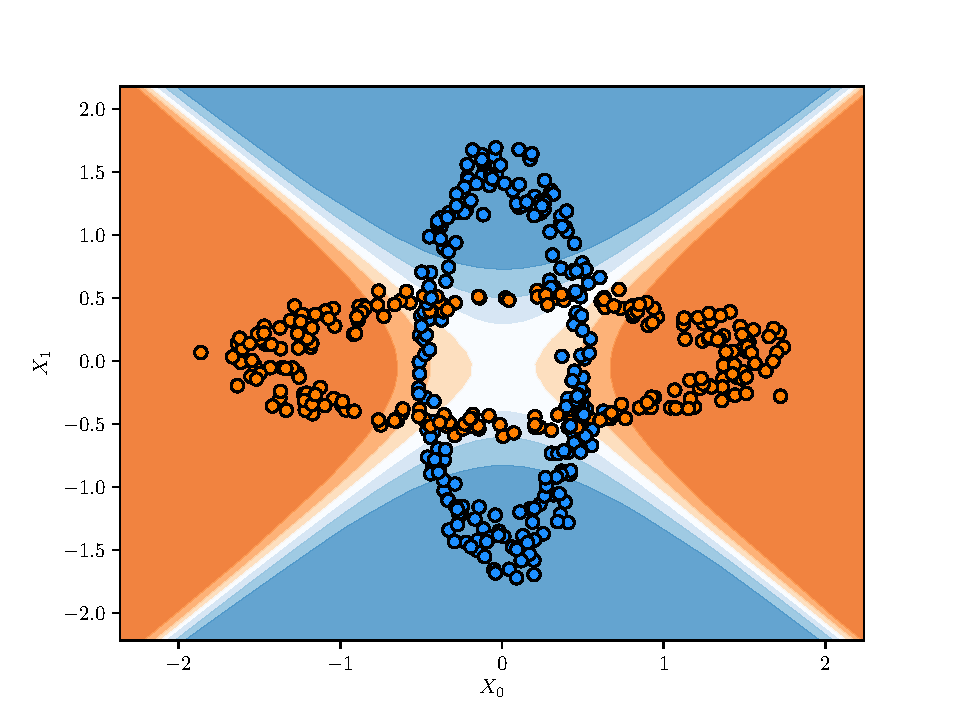
\includegraphics[width=\textwidth]{resources/pdf/make_data1_gnb.pdf}
        \caption{Dataset 1 (\texttt{make\_data1})}
    \end{subfigure}
    \begin{subfigure}{0.495\textwidth}
        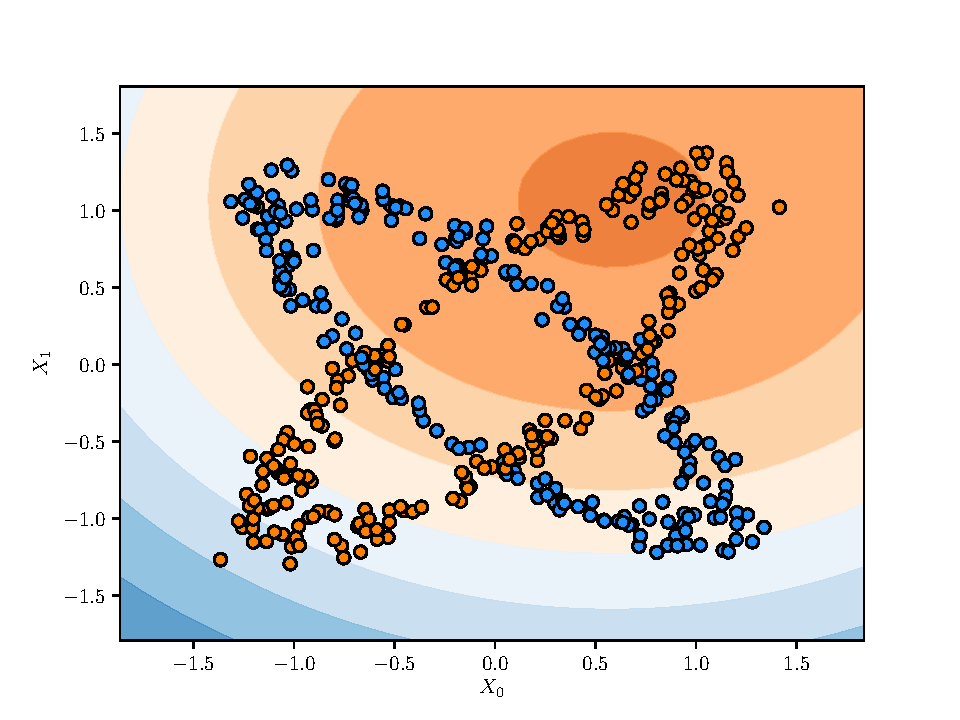
\includegraphics[width=\textwidth]{resources/pdf/make_data2_gnb.pdf}
        \caption{Dataset 2 (\texttt{make\_data2})}
    \end{subfigure}
    \noskipcaption{Decision boundary for Naive Bayes classifier algorithm for both datasets}
    \label{fig:gnb}
\end{figure}
The accuracies computed for each testing set are presented in table \ref{tab:gnb_accuracies}.
\begin{table}[H]
    \centering
    \begin{tabular}{|c|c|}
        \hline
        {\bf Dataset 1} & {\bf Dataset 2}\\ \hline
        \hline
        \num{0.7978} & \num{0.5535} \\ \hline
    \end{tabular}
    \caption{Testing set accuracy for both datasets.}
    \label{tab:gnb_accuracies}
\end{table}
Based on figure \ref{fig:gnb}, we see that the estimator gives satisfactory results for dataset 1 but poor results for dataset 2. This finding is reinforced by the computed scores : not far from \num{80}\% accuracy for dataset 1 against just above \num{50}\% for dataset 2.\par
One reason for that might be that the \og{}mixing zone\fg{} (\textit{i.e.} the central rhombus in which the two classes of points are present) is bigger for dataset 2, and so the probability densities of the two classes are not as clearly separable as for dataset 1. If we look closely at the statisical values of the two datasets, we see that the two classes of the second dataset have almost the same means and almost the same variances along the 2 axes, whereas the variances for the first dataset are much more different, and so the naive Bayes classification works better on the first dataset. Indeed, the choice to presume Gaussianity for the likelihood makes it so that the values of the means and variances for the two classes impact greatly the accuracy of the algorithm. Having them too close leads to poor performances.
